% GNUPLOT: LaTeX picture with Postscript
\begingroup
  \makeatletter
  \providecommand\color[2][]{%
    \GenericError{(gnuplot) \space\space\space\@spaces}{%
      Package color not loaded in conjunction with
      terminal option `colourtext'%
    }{See the gnuplot documentation for explanation.%
    }{Either use 'blacktext' in gnuplot or load the package
      color.sty in LaTeX.}%
    \renewcommand\color[2][]{}%
  }%
  \providecommand\includegraphics[2][]{%
    \GenericError{(gnuplot) \space\space\space\@spaces}{%
      Package graphicx or graphics not loaded%
    }{See the gnuplot documentation for explanation.%
    }{The gnuplot epslatex terminal needs graphicx.sty or graphics.sty.}%
    \renewcommand\includegraphics[2][]{}%
  }%
  \providecommand\rotatebox[2]{#2}%
  \@ifundefined{ifGPcolor}{%
    \newif\ifGPcolor
    \GPcolorfalse
  }{}%
  \@ifundefined{ifGPblacktext}{%
    \newif\ifGPblacktext
    \GPblacktexttrue
  }{}%
  % define a \g@addto@macro without @ in the name:
  \let\gplgaddtomacro\g@addto@macro
  % define empty templates for all commands taking text:
  \gdef\gplbacktext{}%
  \gdef\gplfronttext{}%
  \makeatother
  \ifGPblacktext
    % no textcolor at all
    \def\colorrgb#1{}%
    \def\colorgray#1{}%
  \else
    % gray or color?
    \ifGPcolor
      \def\colorrgb#1{\color[rgb]{#1}}%
      \def\colorgray#1{\color[gray]{#1}}%
      \expandafter\def\csname LTw\endcsname{\color{white}}%
      \expandafter\def\csname LTb\endcsname{\color{black}}%
      \expandafter\def\csname LTa\endcsname{\color{black}}%
      \expandafter\def\csname LT0\endcsname{\color[rgb]{1,0,0}}%
      \expandafter\def\csname LT1\endcsname{\color[rgb]{0,1,0}}%
      \expandafter\def\csname LT2\endcsname{\color[rgb]{0,0,1}}%
      \expandafter\def\csname LT3\endcsname{\color[rgb]{1,0,1}}%
      \expandafter\def\csname LT4\endcsname{\color[rgb]{0,1,1}}%
      \expandafter\def\csname LT5\endcsname{\color[rgb]{1,1,0}}%
      \expandafter\def\csname LT6\endcsname{\color[rgb]{0,0,0}}%
      \expandafter\def\csname LT7\endcsname{\color[rgb]{1,0.3,0}}%
      \expandafter\def\csname LT8\endcsname{\color[rgb]{0.5,0.5,0.5}}%
    \else
      % gray
      \def\colorrgb#1{\color{black}}%
      \def\colorgray#1{\color[gray]{#1}}%
      \expandafter\def\csname LTw\endcsname{\color{white}}%
      \expandafter\def\csname LTb\endcsname{\color{black}}%
      \expandafter\def\csname LTa\endcsname{\color{black}}%
      \expandafter\def\csname LT0\endcsname{\color{black}}%
      \expandafter\def\csname LT1\endcsname{\color{black}}%
      \expandafter\def\csname LT2\endcsname{\color{black}}%
      \expandafter\def\csname LT3\endcsname{\color{black}}%
      \expandafter\def\csname LT4\endcsname{\color{black}}%
      \expandafter\def\csname LT5\endcsname{\color{black}}%
      \expandafter\def\csname LT6\endcsname{\color{black}}%
      \expandafter\def\csname LT7\endcsname{\color{black}}%
      \expandafter\def\csname LT8\endcsname{\color{black}}%
    \fi
  \fi
  \setlength{\unitlength}{0.0500bp}%
  \begin{picture}(8502.00,5102.00)%
    \gplgaddtomacro\gplbacktext{%
      \csname LTb\endcsname%
      \put(814,704){\makebox(0,0)[r]{\strut{}0.0}}%
      \put(814,1279){\makebox(0,0)[r]{\strut{}1.0}}%
      \put(814,1854){\makebox(0,0)[r]{\strut{}2.0}}%
      \put(814,2429){\makebox(0,0)[r]{\strut{}3.0}}%
      \put(814,3004){\makebox(0,0)[r]{\strut{}4.0}}%
      \put(814,3579){\makebox(0,0)[r]{\strut{}5.0}}%
      \put(814,4154){\makebox(0,0)[r]{\strut{}6.0}}%
      \put(946,484){\makebox(0,0){\strut{}0.0}}%
      \put(1741,484){\makebox(0,0){\strut{}0.5}}%
      \put(2537,484){\makebox(0,0){\strut{}1.0}}%
      \put(3332,484){\makebox(0,0){\strut{}1.5}}%
      \put(4128,484){\makebox(0,0){\strut{}2.0}}%
      \put(4923,484){\makebox(0,0){\strut{}2.5}}%
      \put(5719,484){\makebox(0,0){\strut{}3.0}}%
      \put(6514,484){\makebox(0,0){\strut{}3.5}}%
      \put(7310,484){\makebox(0,0){\strut{}4.0}}%
      \put(8105,484){\makebox(0,0){\strut{}4.5}}%
      \put(176,2572){\rotatebox{-270}{\makebox(0,0){\strut{}$f_N \ [Hz]$}}}%
      \put(4525,154){\makebox(0,0){\strut{}$f_K \ [Hz]$}}%
      \put(4525,4771){\makebox(0,0){\strut{}Nutation in Abhängigkeit der Kreiselfrequenz $f_N(f_K)$}}%
      \put(1344,3579){\makebox(0,0)[l]{\strut{}$a\pm \Delta a = 1.513 \pm 0.017 $}}%
    }%
    \gplgaddtomacro\gplfronttext{%
      \csname LTb\endcsname%
      \put(2266,4268){\makebox(0,0)[r]{\strut{}Messwerte}}%
      \csname LTb\endcsname%
      \put(2266,4048){\makebox(0,0)[r]{\strut{}$f(x) = ax$}}%
    }%
    \gplbacktext
    \put(0,0){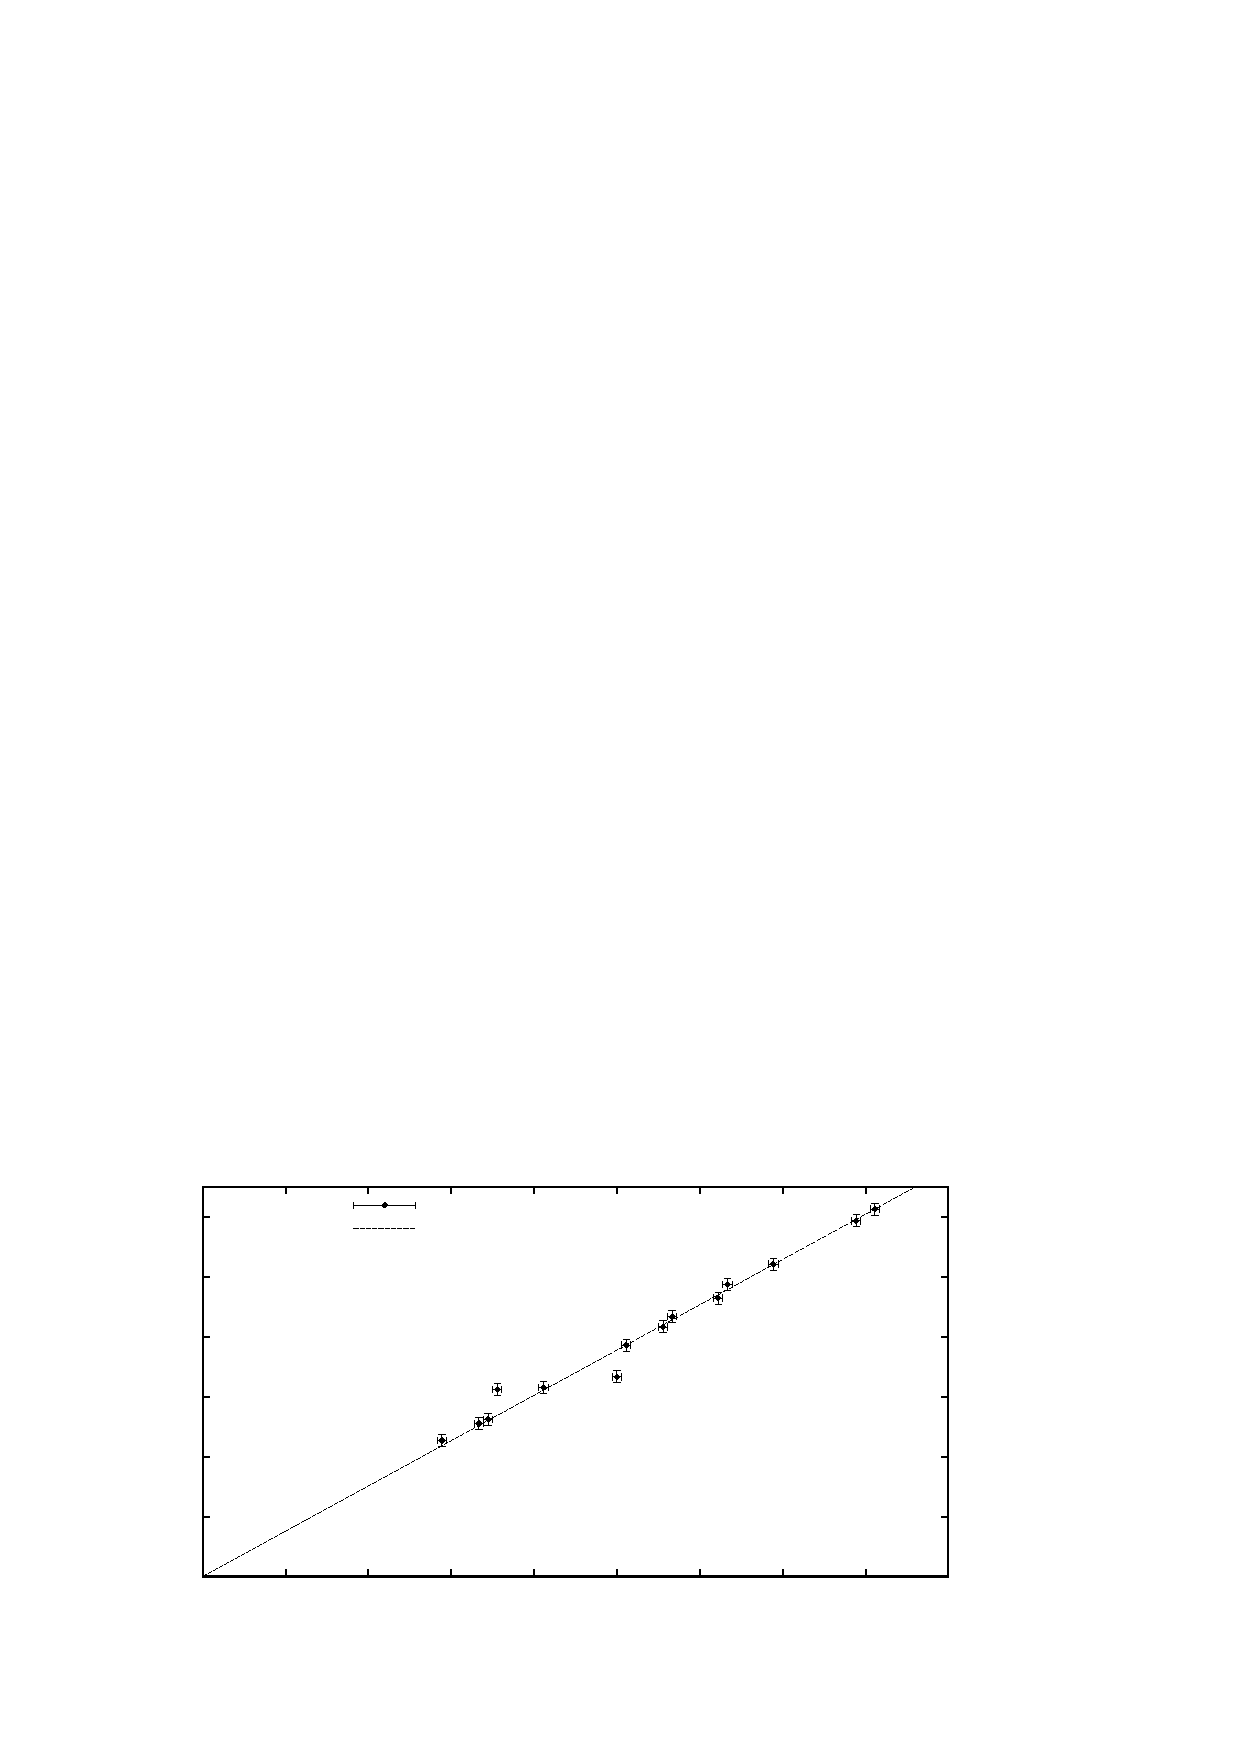
\includegraphics{nutation}}%
    \gplfronttext
  \end{picture}%
\endgroup
